\documentclass[12pt, answers]{exam}
\usepackage[a4paper, hmargin=0.75in, top=1in, bottom=0.2in]{geometry}
\usepackage{amsmath, amssymb}
\usepackage{graphicx}
\usepackage{hyperref}
\usepackage{graphicx}

\begin{document}

\section*{Part 1}

I choose to analysis the League of Legends dataset, and I choose this dataset because I have recently started playing the game due to the new show Arcane on Netflix. I hope by analyzing this dataset I can learn more about the game and improve my gameplay, hopefully see how early gameplay can affect the outcome of the game.

\section*{Part 2}
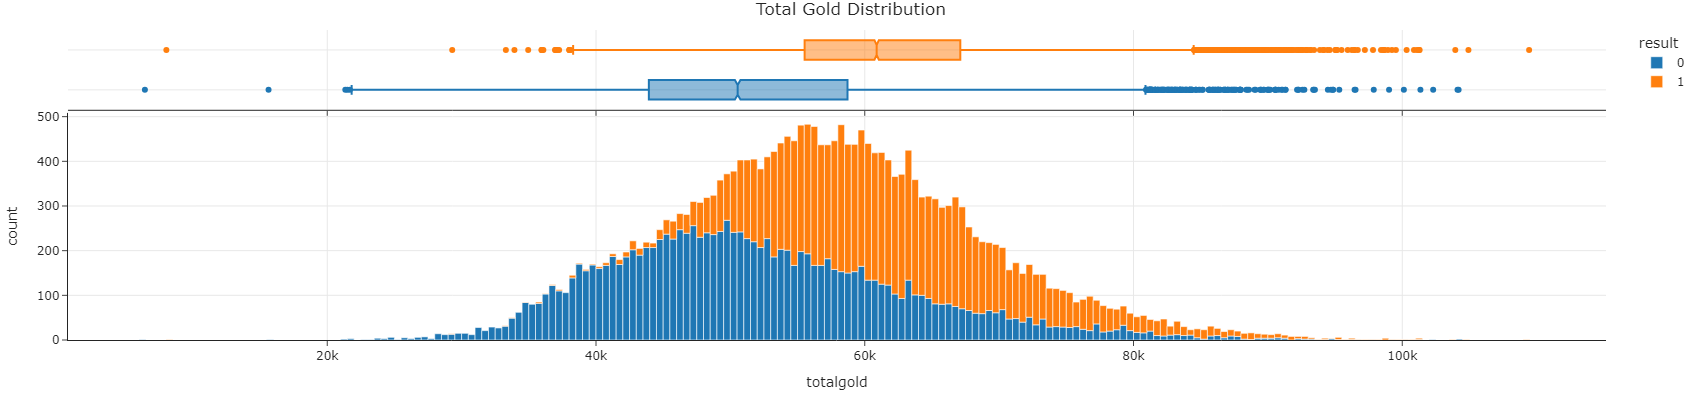
\includegraphics[scale=.275]{totalGoldDistrubution.png}

\section*{Part 3}
The column that I plan to analyze is the total gold column and potentialy the gold per minute column. I plan to analyze the total gold column because I think it is a good indicator of how well a player is doing in the game. I also plan to analyze the gold per minute column because I think it is a good indicator of how well a player is doing in the game over time. I plan to use the total gold column to see if there is a correlation between the total gold and the outcome of the game. I also plan to use the gold per minute column to see if there is a correlation between the gold per minute and the outcome of the game. This problem is considered a classification because I am trying to classify the outcome of the game based on the total gold and gold per minute. 

\end{document}